% Options for packages loaded elsewhere
\PassOptionsToPackage{unicode}{hyperref}
\PassOptionsToPackage{hyphens}{url}
%
\documentclass[
  8pt,
  ignorenonframetext,
]{beamer}
\author{}
\date{\vspace{-2.5em}}

\usepackage{pgfpages}
\setbeamertemplate{caption}[numbered]
\setbeamertemplate{caption label separator}{: }
\setbeamercolor{caption name}{fg=normal text.fg}
\beamertemplatenavigationsymbolsempty
% Prevent slide breaks in the middle of a paragraph
\widowpenalties 1 10000
\raggedbottom
\setbeamertemplate{part page}{
  \centering
  \begin{beamercolorbox}[sep=16pt,center]{part title}
    \usebeamerfont{part title}\insertpart\par
  \end{beamercolorbox}
}
\setbeamertemplate{section page}{
  \centering
  \begin{beamercolorbox}[sep=12pt,center]{part title}
    \usebeamerfont{section title}\insertsection\par
  \end{beamercolorbox}
}
\setbeamertemplate{subsection page}{
  \centering
  \begin{beamercolorbox}[sep=8pt,center]{part title}
    \usebeamerfont{subsection title}\insertsubsection\par
  \end{beamercolorbox}
}
\AtBeginPart{
  \frame{\partpage}
}
\AtBeginSection{
  \ifbibliography
  \else
    \frame{\sectionpage}
  \fi
}
\AtBeginSubsection{
  \frame{\subsectionpage}
}
\usepackage{amsmath,amssymb}
\usepackage{lmodern}
\usepackage{iftex}
\ifPDFTeX
  \usepackage[T1]{fontenc}
  \usepackage[utf8]{inputenc}
  \usepackage{textcomp} % provide euro and other symbols
\else % if luatex or xetex
  \usepackage{unicode-math}
  \defaultfontfeatures{Scale=MatchLowercase}
  \defaultfontfeatures[\rmfamily]{Ligatures=TeX,Scale=1}
\fi
% Use upquote if available, for straight quotes in verbatim environments
\IfFileExists{upquote.sty}{\usepackage{upquote}}{}
\IfFileExists{microtype.sty}{% use microtype if available
  \usepackage[]{microtype}
  \UseMicrotypeSet[protrusion]{basicmath} % disable protrusion for tt fonts
}{}
\makeatletter
\@ifundefined{KOMAClassName}{% if non-KOMA class
  \IfFileExists{parskip.sty}{%
    \usepackage{parskip}
  }{% else
    \setlength{\parindent}{0pt}
    \setlength{\parskip}{6pt plus 2pt minus 1pt}}
}{% if KOMA class
  \KOMAoptions{parskip=half}}
\makeatother
\usepackage{xcolor}
\IfFileExists{xurl.sty}{\usepackage{xurl}}{} % add URL line breaks if available
\IfFileExists{bookmark.sty}{\usepackage{bookmark}}{\usepackage{hyperref}}
\hypersetup{
  hidelinks,
  pdfcreator={LaTeX via pandoc}}
\urlstyle{same} % disable monospaced font for URLs
\newif\ifbibliography
\usepackage{color}
\usepackage{fancyvrb}
\newcommand{\VerbBar}{|}
\newcommand{\VERB}{\Verb[commandchars=\\\{\}]}
\DefineVerbatimEnvironment{Highlighting}{Verbatim}{commandchars=\\\{\}}
% Add ',fontsize=\small' for more characters per line
\usepackage{framed}
\definecolor{shadecolor}{RGB}{248,248,248}
\newenvironment{Shaded}{\begin{snugshade}}{\end{snugshade}}
\newcommand{\AlertTok}[1]{\textcolor[rgb]{0.94,0.16,0.16}{#1}}
\newcommand{\AnnotationTok}[1]{\textcolor[rgb]{0.56,0.35,0.01}{\textbf{\textit{#1}}}}
\newcommand{\AttributeTok}[1]{\textcolor[rgb]{0.77,0.63,0.00}{#1}}
\newcommand{\BaseNTok}[1]{\textcolor[rgb]{0.00,0.00,0.81}{#1}}
\newcommand{\BuiltInTok}[1]{#1}
\newcommand{\CharTok}[1]{\textcolor[rgb]{0.31,0.60,0.02}{#1}}
\newcommand{\CommentTok}[1]{\textcolor[rgb]{0.56,0.35,0.01}{\textit{#1}}}
\newcommand{\CommentVarTok}[1]{\textcolor[rgb]{0.56,0.35,0.01}{\textbf{\textit{#1}}}}
\newcommand{\ConstantTok}[1]{\textcolor[rgb]{0.00,0.00,0.00}{#1}}
\newcommand{\ControlFlowTok}[1]{\textcolor[rgb]{0.13,0.29,0.53}{\textbf{#1}}}
\newcommand{\DataTypeTok}[1]{\textcolor[rgb]{0.13,0.29,0.53}{#1}}
\newcommand{\DecValTok}[1]{\textcolor[rgb]{0.00,0.00,0.81}{#1}}
\newcommand{\DocumentationTok}[1]{\textcolor[rgb]{0.56,0.35,0.01}{\textbf{\textit{#1}}}}
\newcommand{\ErrorTok}[1]{\textcolor[rgb]{0.64,0.00,0.00}{\textbf{#1}}}
\newcommand{\ExtensionTok}[1]{#1}
\newcommand{\FloatTok}[1]{\textcolor[rgb]{0.00,0.00,0.81}{#1}}
\newcommand{\FunctionTok}[1]{\textcolor[rgb]{0.00,0.00,0.00}{#1}}
\newcommand{\ImportTok}[1]{#1}
\newcommand{\InformationTok}[1]{\textcolor[rgb]{0.56,0.35,0.01}{\textbf{\textit{#1}}}}
\newcommand{\KeywordTok}[1]{\textcolor[rgb]{0.13,0.29,0.53}{\textbf{#1}}}
\newcommand{\NormalTok}[1]{#1}
\newcommand{\OperatorTok}[1]{\textcolor[rgb]{0.81,0.36,0.00}{\textbf{#1}}}
\newcommand{\OtherTok}[1]{\textcolor[rgb]{0.56,0.35,0.01}{#1}}
\newcommand{\PreprocessorTok}[1]{\textcolor[rgb]{0.56,0.35,0.01}{\textit{#1}}}
\newcommand{\RegionMarkerTok}[1]{#1}
\newcommand{\SpecialCharTok}[1]{\textcolor[rgb]{0.00,0.00,0.00}{#1}}
\newcommand{\SpecialStringTok}[1]{\textcolor[rgb]{0.31,0.60,0.02}{#1}}
\newcommand{\StringTok}[1]{\textcolor[rgb]{0.31,0.60,0.02}{#1}}
\newcommand{\VariableTok}[1]{\textcolor[rgb]{0.00,0.00,0.00}{#1}}
\newcommand{\VerbatimStringTok}[1]{\textcolor[rgb]{0.31,0.60,0.02}{#1}}
\newcommand{\WarningTok}[1]{\textcolor[rgb]{0.56,0.35,0.01}{\textbf{\textit{#1}}}}
\usepackage{longtable,booktabs,array}
\usepackage{calc} % for calculating minipage widths
\usepackage{caption}
% Make caption package work with longtable
\makeatletter
\def\fnum@table{\tablename~\thetable}
\makeatother
\setlength{\emergencystretch}{3em} % prevent overfull lines
\providecommand{\tightlist}{%
  \setlength{\itemsep}{0pt}\setlength{\parskip}{0pt}}
\setcounter{secnumdepth}{-\maxdimen} % remove section numbering
% type setting
% ------------------------------------------------------------------------------
\usepackage[german]{babel}     

% fonts
% ------------------------------------------------------------------------------
\usefonttheme{professionalfonts}

% slide title and horizontal line
% ------------------------------------------------------------------------------
\setbeamertemplate{frametitle}{%
    \vskip-30pt \color{black}\large%
    \begin{minipage}[b][23pt]{120mm}%
    \flushleft\insertframetitle%
    \end{minipage}%
}

\setbeamertemplate{headline}										
{
\vskip10pt\hfill\hspace{3.5mm} 										 
\vskip15pt\color{black}\rule{\textwidth}{0.4pt} 					 
}

% slide number
% ---------------------------------------------------------------
\setbeamertemplate{navigation symbols}{}
\setbeamertemplate{footline}
{
\vskip5pt
\vskip2pt
\makebox[123mm]{\hspace{7.5mm}
\hfill Allgemeines lineares Modell $\vert$ 
\copyright $ $ 2022 Dirk Ostwald CC BY-NC-SA 4.0 $\vert$ 
Folie \insertframenumber}
\vskip4pt
}

% block color scheme
% ------------------------------------------------------------------------------
% colors
\definecolor{white}{RGB}{255,255,255}
\definecolor{grey}{RGB}{235,235,235}
\definecolor{lightgrey}{RGB}{245,245,245}
\definecolor{LightBlue}{RGB}{220,220,255}
\definecolor{darkblue}{RGB}{51, 51, 153}

% definitions and theorems
\setbeamercolor{block title}{fg = black, bg = grey}
\setbeamercolor{block body}{fg = black, bg = lightgrey}

% general line spacing 
% ------------------------------------------------------------------------------
\linespread{1.3}

% local line spacing
% ------------------------------------------------------------------------------
\usepackage{setspace}

% colors
% -----------------------------------------------------------------------------
\usepackage{color}

% justified text
% ------------------------------------------------------------------------------
\usepackage{ragged2e}
\usepackage{etoolbox}
\apptocmd{\frame}{}{\justifying}{}

% bullet point lists
% -----------------------------------------------------------------------------
\setbeamertemplate{itemize item}[circle]
\setbeamertemplate{itemize subitem}[circle]
\setbeamertemplate{itemize subsubitem}[circle]
\setbeamercolor{itemize item}{fg = black}
\setbeamercolor{itemize subitem}{fg = black}
\setbeamercolor{itemize subsubitem}{fg = black}
\setbeamercolor{enumerate item}{fg = black}
\setbeamercolor{enumerate subitem}{fg = black}
\setbeamercolor{enumerate subsubitem}{fg = black}
\setbeamerfont{itemize/enumerate body}{}
\setbeamerfont{itemize/enumerate subbody}{size = \normalsize}
\setbeamerfont{itemize/enumerate subsubbody}{size = \normalsize}

% color links
% ------------------------------------------------------------------------------
\usepackage{hyperref}
\definecolor{urls}{RGB}{204,0,0}
\hypersetup{colorlinks, citecolor = darkblue, urlcolor = urls}


% additional math commands
% ------------------------------------------------------------------------------
\usepackage{bm}                                         
\newcommand{\niton}{\not\owns}
\DeclareMathOperator*{\intinf}{\int_{-\infty}^{\infty}}


% text highlighting
% ------------------------------------------------------------------------------
\usepackage{soul}
\makeatletter
\let\HL\hl
\renewcommand\hl{%
  \let\set@color\beamerorig@set@color
  \let\reset@color\beamerorig@reset@color
  \HL}
\makeatother

% equation highlighting
% -----------------------------------------------------------------------------
\newcommand{\highlight}[2][yellow]{\mathchoice%
  {\colorbox{#1}{$\displaystyle#2$}}%
  {\colorbox{#1}{$\textstyle#2$}}%
  {\colorbox{#1}{$\scriptstyle#2$}}%
  {\colorbox{#1}{$\scriptscriptstyle#2$}}}%

% additional mathematical operators
% ------------------------------------------------------------------------------
\DeclareMathOperator*{\argmax}{arg\,max}
\DeclareMathOperator*{\argmin}{arg\,min}

\ifLuaTeX
  \usepackage{selnolig}  % disable illegal ligatures
\fi

\begin{document}

\begin{frame}[plain]{}
\protect\hypertarget{section}{}
\center

\begin{center}
\includegraphics[width=0.2\linewidth]{1_Abbildungen/alm_1_otto} \end{center}

\vspace{2mm}

\huge

Allgemeines Lineares Modell \vspace{6mm}

\large

BSc Psychologie SoSe 2022

\vspace{6mm}
\normalsize

Prof.~Dr.~Dirk Ostwald
\end{frame}

\begin{frame}[plain]{}
\protect\hypertarget{section-1}{}
\center
\huge
\vfill

\noindent (1) Regression \vfill
\end{frame}

\begin{frame}{}
\protect\hypertarget{section-2}{}
\setstretch{3}
\vfill
\large

Methode der kleinsten Quadrate

Einfache lineare Regression

Selbstkontrollfragen

\vfill
\end{frame}

\begin{frame}{}
\protect\hypertarget{section-3}{}
\setstretch{3}
\vfill
\large

\textbf{Methode der kleinsten Quadrate}

Einfache lineare Regression

Selbstkontrollfragen

\vfill
\end{frame}

\begin{frame}{Methode der kleinsten Quadrate}
\protect\hypertarget{methode-der-kleinsten-quadrate}{}
\large

Anwendungsszenario \vspace{2mm}

\begin{center}
\includegraphics[width=0.8\linewidth]{1_Abbildungen/alm_1_beispielszenario} \end{center}
\end{frame}

\begin{frame}{Methode der kleinsten Quadrate}
\protect\hypertarget{methode-der-kleinsten-quadrate-1}{}
Beispieldatensatz

\center
\footnotesize

\(i = 1,...,20\) Patient:innen, \(y_i\) Symptomreduktion bei Patient:in
\(i\), \(x_i\) Anzahl Therapiestunden von Patient:in \(i\)

\setstretch{1}

\begin{longtable}[]{@{}rr@{}}
\toprule
y\_i & x\_i \\
\midrule
\endhead
-3.15 & 1 \\
2.52 & 2 \\
-1.18 & 3 \\
3.06 & 4 \\
1.70 & 5 \\
2.91 & 6 \\
3.92 & 7 \\
2.31 & 8 \\
4.63 & 9 \\
10.91 & 10 \\
17.56 & 11 \\
11.52 & 12 \\
12.31 & 13 \\
12.12 & 14 \\
12.13 & 15 \\
20.37 & 16 \\
25.26 & 17 \\
27.75 & 18 \\
24.93 & 19 \\
32.49 & 20 \\
\bottomrule
\end{longtable}
\end{frame}

\begin{frame}{Methode der kleinsten Quadrate}
\protect\hypertarget{methode-der-kleinsten-quadrate-2}{}
Beispieldatensatz

\begin{center}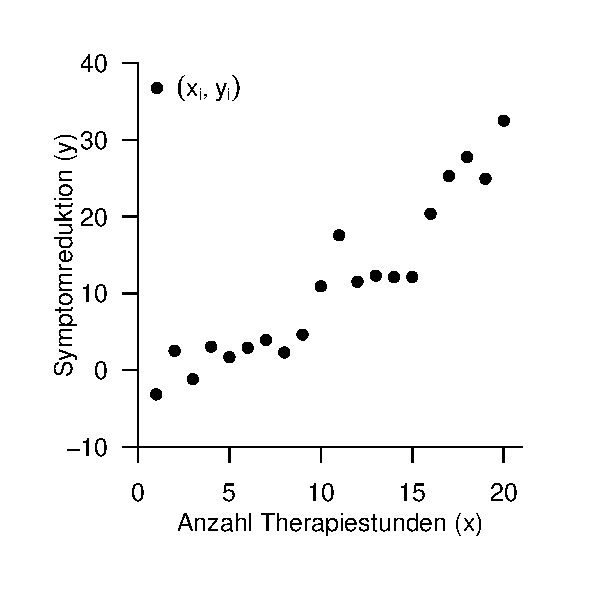
\includegraphics[width=0.55\linewidth]{1_Abbildungen/alm_1_beispieldatensatz} \end{center}

\center

\textcolor{darkblue}{Welcher funktionaler Zusammenhang zwischen $x$ und $y$ liegt den Daten zugrunde?}
\end{frame}

\begin{frame}{Methode der kleinsten Quadrate}
\protect\hypertarget{methode-der-kleinsten-quadrate-3}{}
\footnotesize
\begin{definition}[Ausgleichsgerade]
\justifying
Für $\beta := (\beta_0,\beta_1)^T \in \mathbb{R}^2$ heißt die linear-affine Funktion
\begin{equation}
f_\beta : \mathbb{R} \to \mathbb{R}, x \mapsto f_\beta(x) := \beta_0 + \beta_1 x,
\end{equation}
für die für eine Wertemenge  $\{(x_1,y_1),...,(x_n,y_n)\} \subset \mathbb{R}^2$ die Funktion
\begin{equation}
q : \mathbb{R}^2 \to \mathbb{R}_{\ge 0}, \beta \mapsto q(\beta)
:= \sum_{i=1}^n (y_i-f_\beta(x_i))^2
 = \sum_{i=1}^n (y_i- (\beta_0 + \beta_1x_i))^2
\end{equation}
der quadrierten vertikalen Abweichungen der $y_i$ von den Funktionswerten $f_{\beta}(x_i)$
ihr Minimum annimt, die \textit{Ausgleichsgerade für die Wertemenge $\{(x_1,y_1),...,(x_n,y_n)\}$}.
\end{definition}

Bemerkungen

\begin{itemize}
\tightlist
\item
  Wir nehmen hier ohne Beweis an, dass das Minimum von \(q\) eindeutig
  ist.
\end{itemize}
\end{frame}

\begin{frame}{Methode der kleinsten Quadrate}
\protect\hypertarget{methode-der-kleinsten-quadrate-4}{}
Linear-affine Funktionen \(f_\beta(x) := \beta_0 + \beta_1 x\)

\small

\begin{itemize}
\tightlist
\item
  \(\beta_0\): Schnittpunkt von Gerade und \(y\)-Achse (``Offset
  Parameter'')
\item
  \(\beta_1\): \(y\)-Differenz pro \(x\)-Einheitsdifferenz
  (``Steigungsparameter'')
\end{itemize}

\vspace{1cm}

\begin{center}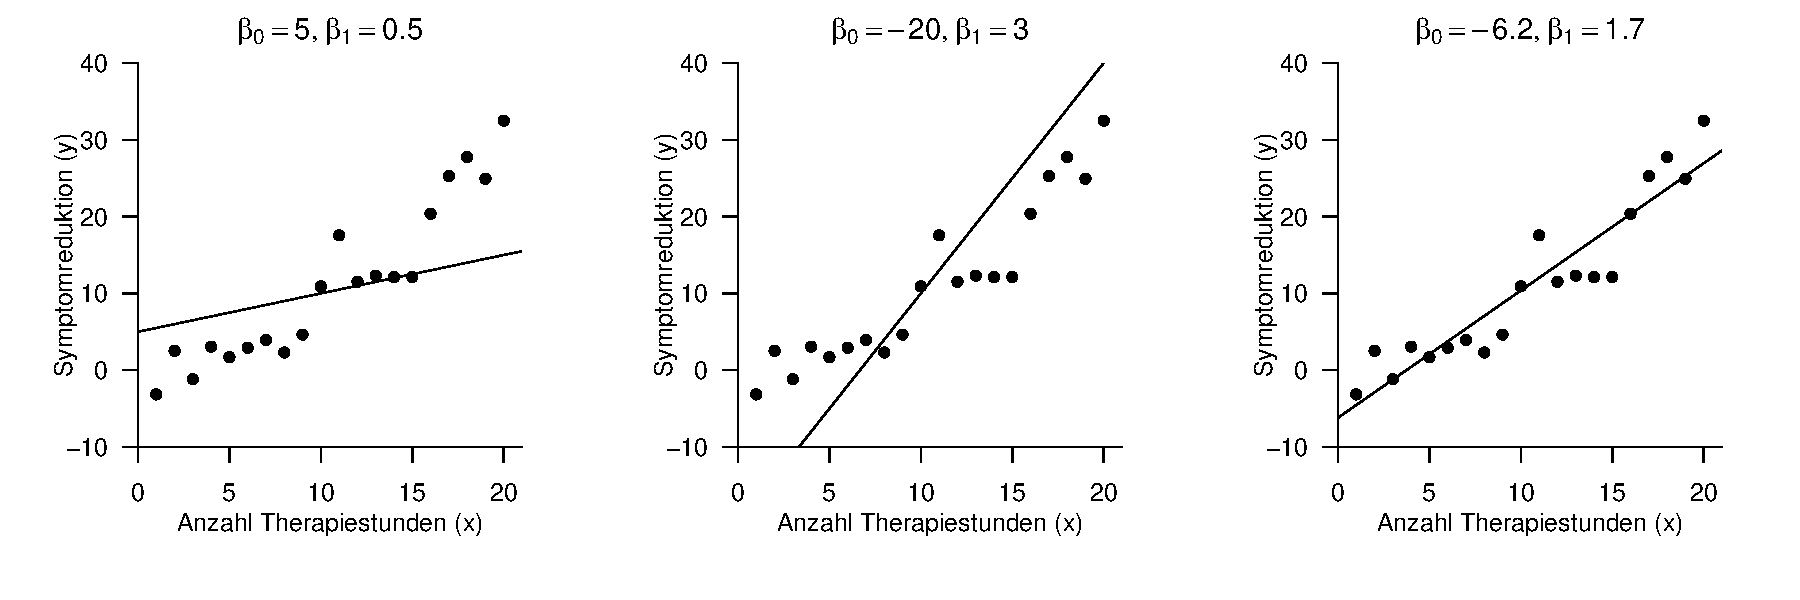
\includegraphics[width=1\linewidth]{1_Abbildungen/alm_1_ausgleichsgerade_1} \end{center}
\end{frame}

\begin{frame}{Methode der kleinsten Quadrate}
\protect\hypertarget{methode-der-kleinsten-quadrate-5}{}
\small

Funktion der quadrierten vertikalen Abweichungen \begin{equation}
q(\beta) := \sum_{i=1}^n (y_i - (\beta_0 + \beta_1x_i))^2
\end{equation}

\begin{center}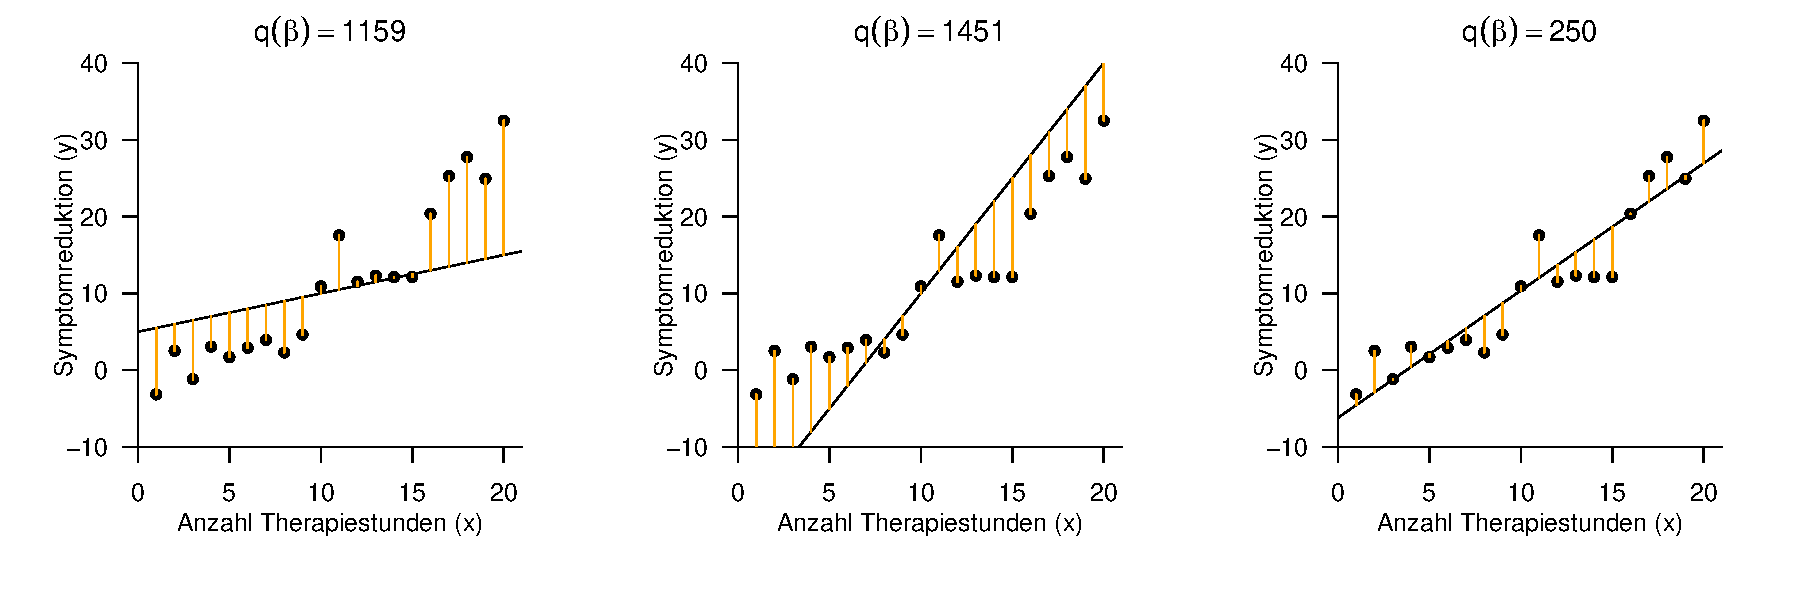
\includegraphics[width=1\linewidth]{1_Abbildungen/alm_1_ausgleichsgerade_2} \end{center}
\center

\textcolor{orange}{\textbf{------}} \(y_i - (\beta_0 + \beta_1x_i)\) für
\(i = 1,...,n\)
\end{frame}

\begin{frame}{Methode der kleinsten Quadrate}
\protect\hypertarget{methode-der-kleinsten-quadrate-6}{}
\footnotesize
\begin{theorem}[Ausgleichsgerade]
\justifying
\normalfont
Für eine Wertemenge $\{(x_1,y_1),...,(x_n,y_n)\}\subset\mathbb{R}^2$ hat die Ausgleichsgerade die Form
\begin{equation}
f_\beta : \mathbb{R} \to \mathbb{R}, x \mapsto f_\beta(x) := \hat{\beta}_0 + \hat{\beta}_1 x,
\end{equation}
wobei mit der Stichprobenkovarianz $c_{xy}$ der $(x_i,y_i)$-Werte, der
Stichprobenvarianz $s_x^2$ der $x_i$-Werte und den Stichprobenmitteln $\bar{x}$
und $\bar{y}$ der $x_i$- und $y_i$-Werte, respektive, gilt, dass
\begin{equation}
\hat{\beta}_1 = \frac{c_{xy}}{s_x^2} \mbox{ und } \hat{\beta}_0 = \bar{y} - \hat{\beta}_1\bar{x}
\end{equation}
\end{theorem}

Bemerkungen

\begin{itemize}
\tightlist
\item
  Mit den Definitionen von \(c_{xy}\) und \(s_x^2\) gilt also
  \begin{equation}
  \hat{\beta}_1 = \frac{\sum_{i=1}^n (x_i - \bar{x})(y_i - \bar{y})}{\sum_{i=1}^n (x_i - \bar{x})^2}
  \end{equation}
\item
  Man spricht hier von der Stichprobenkovarianz \(c_{xy}\), auch wenn
  die Werte \(x_1,...,x_n\) oft nicht als Realisierungen einer
  Stichprobe \(X_1,...,X_n\) verstanden werden, sondern als gegebene
  oder selbst gewählte Zahlen.
\end{itemize}
\end{frame}

\begin{frame}{Methode der kleinsten Quadrate}
\protect\hypertarget{methode-der-kleinsten-quadrate-7}{}
\tiny
\setlength{\abovedisplayskip}{3pt}
\setlength{\belowdisplayskip}{3pt}
\setstretch{1.2}

\underline{Beweis}

Wir betrachten die Summe der quadrierten vertikalen Abweichungen der
\(y_i\) von den Funktionswerten \(f(x_i)\) als Funktion von \(\beta_0\)
und \(\beta_1\) und bestimmen Werte \(\hat{\beta}_0\) und
\(\hat{\beta}_1\), für die diese Funktion ihr Minimum annimmt, die Summe
der quadrierten vertikalen Abweichungen der \(y_i\) von den
Funktionswerten \(f(x_i)\) also minimal ist. Wir betrachten also die
Funktion \begin{equation}
q : \mathbb{R}^2 \to \mathbb{R}, (\beta_0,\beta_1) \mapsto q(\beta_0,\beta_1)
:= \sum_{i=1}^n \left(y_i - (\beta_0 + \beta_1 x)\right)^2.
\end{equation} Um das Minimum dieser Funktion zu bestimmen, berechnen
wir zunächst die partiellen Ableitungen hinsichtlich \(\beta_0\) und
\(\beta_1\) und setzen diese gleich 0. Es ergibt sich zunächst
\begin{align}
\begin{split}
\frac{\partial}{\partial \beta_0} q(\beta_0,\beta_1)
& = \frac{\partial}{\partial \beta_0}\left(\sum_{i=1}^n \left(y_i - (\beta_0 + \beta_1 x_i)\right)^2\right) \\[-5pt]
& = \sum_{i=1}^n \frac{\partial}{\partial \beta_0} \left(y_i - (\beta_0 + \beta_1 x_i)\right)^2 \\[-5pt]
& = \sum_{i=1}^n 2\left(y_i - (\beta_0 + \beta_1 x_i)\right)\frac{\partial}{\partial \beta_0}\left(y_i - \beta_0 - \beta_1 x_i \right)  \\[-5pt]
&  = -2\sum_{i=1}^n \left(y_i - \beta_0  - \beta_1 x_i\right)
\end{split}
\end{align}
\end{frame}

\begin{frame}{Methode der kleinsten Quadrate}
\protect\hypertarget{methode-der-kleinsten-quadrate-8}{}
\tiny
\setlength{\abovedisplayskip}{3pt}
\setlength{\belowdisplayskip}{3pt}
\setstretch{1.2}
\vspace{3mm}

\underline{Beweis (fortgeführt)}

Weiterhin ergibt sich \vspace{-2mm} \begin{align}
\begin{split}
\frac{\partial}{\partial \beta_1} q(\beta_0,\beta_1)
& = \frac{\partial}{\partial \beta_1}\left(\sum_{i=1}^n \left(y_i - (\beta_0 + \beta_1 x_i)\right)^2\right) \\[-5pt]
& = \sum_{i=1}^n \frac{\partial}{\partial \beta_1} \left(y_i - (\beta_0 + \beta_1 x_i)\right)^2 \\[-5pt]
& = \sum_{i=1}^n 2\left(y_i - (\beta_0 + \beta_1 x_i)\right)\frac{\partial}{\partial \beta_1}\left(y_i - \beta_0 - \beta_1 x_i \right) \\[-5pt]
& = -2\sum_{i=1}^n \left(y_i - \beta_0  - \beta_1 x_i\right)x_i
\end{split}
\end{align} Nullsetzen beider partieller Ableitungen ergibt dann
\begin{align}
\begin{split}
\frac{\partial}{\partial \beta_0} q(\beta_0,\beta_1)  = 0       & \mbox{ und }
\frac{\partial}{\partial \beta_1} q(\beta_0,\beta_1)  = 0
\\[-5pt]
\Leftrightarrow
-2\sum_{i=1}^n \left(y_i - \beta_0  - \beta_1 x_i\right)    = 0 & \mbox{ und }
-2\sum_{i=1}^n \left(y_i - \beta_0  - \beta_1 x_i\right)x_i = 0
\\[-5pt]
\Leftrightarrow
\sum_{i=1}^n \left(y_i - \beta_0  - \beta_1 x_i\right)       = 0 & \mbox{ und }
\sum_{i=1}^n \left(y_i - \beta_0  - \beta_1 x_i\right)x_i    = 0
\end{split}
\end{align}
\end{frame}

\begin{frame}{Methode der kleinsten Quadrate}
\protect\hypertarget{methode-der-kleinsten-quadrate-9}{}
\tiny
\setlength{\abovedisplayskip}{3pt}
\setlength{\belowdisplayskip}{3pt}
\setstretch{1.2}

\underline{Beweis (fortgeführt)}

und weiter \vspace{-2mm} \begin{align}
\begin{split}
\sum_{i=1}^n y_i    - \sum_{i=1}^n \beta_0     - \beta_1 \sum_{i=1}^n x_i    = 0 & \mbox{ und }
\sum_{i=1}^n y_ix_i - \sum_{i=1}^n \beta_0x_i  - \beta_1 \sum_{i=1}^n x_i^2  = 0 \\[-5pt]
\Leftrightarrow
\beta_0n  + \beta_1 \sum_{i=1}^n x_i    = \sum_{i=1}^n y_i & \mbox{ und }
\beta_0\sum_{i=1}^n x_i  + \beta_1 \sum_{i=1}^n x_i^2  = \sum_{i=1}^n y_ix_i
\end{split}
\end{align} Das sich hier ergebende Gleichungssystem \begin{align}
\begin{split}
\beta_0 n                + \beta_1 \sum_{i=1}^n x_i    & = \sum_{i=1}^n y_i    \\[-5pt]
\beta_0 \sum_{i=1}^n x_i + \beta_1 \sum_{i=1}^n x_i^2  & = \sum_{i=1}^n y_ix_i
\end{split}
\end{align} wird \textit{System der Normalengleichungen} genannt und
beschreibt die notwendige Bedingung für ein Minimum von \(q\). Auflösen
dieses Gleichungssystems nach \(\beta_0\) und \(\beta_1\) liefert dann
die Werte \(\hat{\beta}_0\) und \(\hat{\beta}_1\) des Theorems.
\end{frame}

\begin{frame}{Methode der kleinsten Quadrate}
\protect\hypertarget{methode-der-kleinsten-quadrate-10}{}
\tiny
\vspace{2mm}
\setlength{\abovedisplayskip}{3pt}
\setlength{\belowdisplayskip}{3pt}
\setstretch{1.1}

\underline{Beweis (fortgeführt)}

Um dies zu sehen, halten wir zunächst fest, dass mit der ersten
Gleichung des Systems der Normalengleichungen gilt \begin{align}
\begin{split}
n\hat{\beta}_0 + \hat{\beta}_1 \sum_{i=1}^n x_i          = \sum_{i=1}^n y_i                 
\Leftrightarrow \hat{\beta}_0 + \hat{\beta}_1\bar{x}     = \bar{y}                          
\Leftrightarrow \hat{\beta}_0                            = \bar{y} - \hat{\beta}_1\bar{x}   
\end{split}
\end{align} Einsetzen der Form von \(\hat{\beta}_0\) in die zweite
Gleichung des Systems der Normalengleichungen ergibt dann zunächst
\begin{align}\label{eq:hat_beta_1}
\begin{split}
\hat{\beta}_0 \sum_{i=1}^n x_i + \hat{\beta}_1 \sum_{i=1}^n x_i^2                                         
& = \sum_{i=1}^n y_ix_i   
\\
\Leftrightarrow
\left(\bar{y} - \hat{\beta}_1\bar{x}\right) \sum_{i=1}^n x_i + \hat{\beta}_1 \sum_{i=1}^n x_i^2           
& = \sum_{i=1}^n y_ix_i   
\\
\Leftrightarrow
\bar{y}\sum_{i=1}^n x_i - \hat{\beta}_1\bar{x}\sum_{i=1}^n x_i  + \hat{\beta}_1 \sum_{i=1}^n x_i^2           
& = \sum_{i=1}^n y_ix_i   
\\
\Leftrightarrow
- \hat{\beta}_1\bar{x}\sum_{i=1}^n x_i  + \hat{\beta}_1 \sum_{i=1}^n x_i^2           
& = \sum_{i=1}^n y_ix_i - \bar{y}\sum_{i=1}^n x_i  
\\
\Leftrightarrow
\hat{\beta}_1 \left(\sum_{i=1}^n x_i^2  - \bar{x}\sum_{i=1}^n x_i\right)         
& = \sum_{i=1}^n y_ix_i - \bar{y}\sum_{i=1}^n x_i  
\end{split}
\end{align}
\end{frame}

\begin{frame}{Methode der kleinsten Quadrate}
\protect\hypertarget{methode-der-kleinsten-quadrate-11}{}
\tiny
\vspace{2mm}
\setlength{\abovedisplayskip}{3pt}
\setlength{\belowdisplayskip}{3pt}
\setstretch{1.1}

\underline{Beweis (fortgeführt)}

Wir halten nun zunächst fest, dass gilt \begin{align}
\begin{split}
\sum_{i=1}^n x_i^2  - \bar{x}\sum_{i=1}^n x_i
& = \sum_{i=1}^n x_i^2 - 2\bar{x}\sum_{i=1}^n x_i + \bar{x}\sum_{i=1}^n x_i \\
& = \sum_{i=1}^n x_i^2 - 2\bar{x}\sum_{i=1}^n x_i + n\left(\frac{1}{n}\sum_{i=1}^n x_i\right)\bar{x} \\
& = \sum_{i=1}^n x_i^2 - 2\bar{x}\sum_{i=1}^n x_i + n\bar{x}^2 \\
& = \sum_{i=1}^n \left(x_i^2 - 2\bar{x} x_i + \bar{x}^2\right) \\
& = \sum_{i=1}^n \left(x_i - \bar{x}\right)^2. \\
\end{split}
\end{align}
\end{frame}

\begin{frame}{Methode der kleinsten Quadrate}
\protect\hypertarget{methode-der-kleinsten-quadrate-12}{}
\tiny
\vspace{2mm}
\setlength{\abovedisplayskip}{3pt}
\setlength{\belowdisplayskip}{3pt}
\setstretch{1.1}

\underline{Beweis (fortgeführt)}

Weiterhin halten wir zunächst fest, dass gilt \begin{align}
\begin{split}
\sum_{i=1}^n y_ix_i - \bar{y}\sum_{i=1}^n x_i 
& = \sum_{i=1}^n y_ix_i - \bar{y}\sum_{i=1}^n x_i - n\bar{y}\bar{x} + n\bar{y}\bar{x}                       \\
& = \sum_{i=1}^n y_ix_i - \bar{y}\sum_{i=1}^n x_i - \sum_{i=1}^n y_i\bar{x}  + \sum_{i=1}^n\bar{y}\bar{x}   \\
& = \sum_{i=1}^n y_ix_i - \sum_{i=1}^n y_i\bar{x} - \sum_{i=1}^n\bar{y} x_i  + \sum_{i=1}^n\bar{y}\bar{x}   \\
& = \sum_{i=1}^n \left(y_ix_i -  y_i\bar{x} - \bar{y} x_i  + \bar{y}\bar{x}\right)                          \\
& = \sum_{i=1}^n \left(y_i-\bar{y}\right)\left(x_i-\bar{x}\right).
\end{split}
\end{align}
\end{frame}

\begin{frame}{Methode der kleinsten Quadrate}
\protect\hypertarget{methode-der-kleinsten-quadrate-13}{}
\tiny
\vspace{2mm}
\setlength{\abovedisplayskip}{3pt}
\setlength{\belowdisplayskip}{3pt}
\setstretch{1.1}

\underline{Beweis (fortgeführt)}

In der Fortsetzung von \eqref{eq:hat_beta_1} ergibt sich dann
\begin{align} 
\begin{split}
\hat{\beta}_1 \left(\sum_{i=1}^n x_i^2  - \bar{x}\sum_{i=1}^n x_i\right)         
& = \sum_{i=1}^n y_ix_i - \bar{y}\sum_{i=1}^n x_i  
\\
\Leftrightarrow
\hat{\beta}_1 \left(\sum_{i=1}^n \left(x_i - \bar{x}\right)^2\right)         
& =  \sum_{i=1}^n \left(y_i-\bar{y}\right)\left(x_i-\bar{x}\right) 
\\
\Leftrightarrow
\hat{\beta}_1        
& = \frac{\sum_{i=1}^n \left(y_i-\bar{y}\right)\left(x_i-\bar{x}\right)}{\sum_{i=1}^n \left(x_i - \bar{x}\right)^2} 
\\
\Leftrightarrow
\hat{\beta}_1        
& = \frac{c_{xy}}{s_x^2}. 
\end{split}
\end{align}

\(\hfill\Box\)
\end{frame}

\begin{frame}[fragile]{Methode der kleinsten Quadrate}
\protect\hypertarget{methode-der-kleinsten-quadrate-14}{}
Beispieldatensatz Analyse \vspace{1mm} \setstretch{1.2}

\footnotesize

\begin{Shaded}
\begin{Highlighting}[]
\CommentTok{\# Einlesen des Beispieldatensatzes}
\NormalTok{fname       }\OtherTok{=} \FunctionTok{file.path}\NormalTok{(}\FunctionTok{getwd}\NormalTok{(), }\StringTok{"1\_Daten"}\NormalTok{, }\StringTok{"1\_Regression.csv"}\NormalTok{)}
\NormalTok{D           }\OtherTok{=} \FunctionTok{read.table}\NormalTok{(fname, }\AttributeTok{sep =} \StringTok{","}\NormalTok{, }\AttributeTok{header =} \ConstantTok{TRUE}\NormalTok{)}

\CommentTok{\# Stichprobenstatistiken}
\NormalTok{x\_bar       }\OtherTok{=} \FunctionTok{mean}\NormalTok{(D}\SpecialCharTok{$}\NormalTok{x\_i)               }\CommentTok{\# Stichprobenmittel der x\_i{-}Werte}
\NormalTok{y\_bar       }\OtherTok{=} \FunctionTok{mean}\NormalTok{(D}\SpecialCharTok{$}\NormalTok{y\_i)               }\CommentTok{\# Stichprobenmittel der y\_i{-}Werte}
\NormalTok{s2x         }\OtherTok{=} \FunctionTok{var}\NormalTok{(D}\SpecialCharTok{$}\NormalTok{x\_i)                }\CommentTok{\# Stichprobenvarianz der  x\_i{-}Werte}
\NormalTok{cxy         }\OtherTok{=} \FunctionTok{cov}\NormalTok{(D}\SpecialCharTok{$}\NormalTok{x\_i, D}\SpecialCharTok{$}\NormalTok{y\_i)         }\CommentTok{\# Stichprobenkovarianz der (x\_i,y\_i){-}Werte}

\CommentTok{\# Ausgleichsgeradenparameter}
\NormalTok{beta\_1\_hat  }\OtherTok{=}\NormalTok{ cxy}\SpecialCharTok{/}\NormalTok{s2x                   }\CommentTok{\# \textbackslash{}hat\{\textbackslash{}beta\}\_1, Steigungsparameter}
\NormalTok{beta\_0\_hat  }\OtherTok{=}\NormalTok{ y\_bar }\SpecialCharTok{{-}}\NormalTok{ beta\_1\_hat}\SpecialCharTok{*}\NormalTok{x\_bar  }\CommentTok{\# \textbackslash{}hat\{\textbackslash{}beta\}\_0, Offset Parameter}

\CommentTok{\# Ausgabe}
\FunctionTok{cat}\NormalTok{(}\StringTok{"beta\_0\_hat:"}\NormalTok{, beta\_0\_hat,}
    \StringTok{"}\SpecialCharTok{\textbackslash{}n}\StringTok{beta\_1\_hat:"}\NormalTok{, beta\_1\_hat)}
\end{Highlighting}
\end{Shaded}

\begin{verbatim}
> beta_0_hat: -6.19 
> beta_1_hat: 1.66
\end{verbatim}
\end{frame}

\begin{frame}[fragile]{Methode der kleinsten Quadrate}
\protect\hypertarget{methode-der-kleinsten-quadrate-15}{}
Beispieldatensatz Visualisierung \vspace{1mm} \setstretch{1.2}

\tiny

\begin{Shaded}
\begin{Highlighting}[]
\CommentTok{\# Datenwerte}
\FunctionTok{plot}\NormalTok{(}
\NormalTok{D}\SpecialCharTok{$}\NormalTok{x\_i,}
\NormalTok{D}\SpecialCharTok{$}\NormalTok{y\_i,}
\AttributeTok{pch         =} \DecValTok{16}\NormalTok{,}
\AttributeTok{xlab        =} \StringTok{"Anzahl Therapiestunden (x)"}\NormalTok{,}
\AttributeTok{ylab        =} \StringTok{"Symptomreduktion (y)"}\NormalTok{,}
\AttributeTok{xlim        =} \FunctionTok{c}\NormalTok{(}\DecValTok{0}\NormalTok{,}\DecValTok{21}\NormalTok{),}
\AttributeTok{ylim        =} \FunctionTok{c}\NormalTok{(}\SpecialCharTok{{-}}\DecValTok{10}\NormalTok{, }\DecValTok{40}\NormalTok{),}
\AttributeTok{main        =} \FunctionTok{TeX}\NormalTok{(}\StringTok{"$}\SpecialCharTok{\textbackslash{}\textbackslash{}}\StringTok{hat\{}\SpecialCharTok{\textbackslash{}\textbackslash{}}\StringTok{beta\}\_0 =  {-}6.19, }\SpecialCharTok{\textbackslash{}\textbackslash{}}\StringTok{hat\{}\SpecialCharTok{\textbackslash{}\textbackslash{}}\StringTok{beta\}\_1 = 1.66$"}\NormalTok{))}

\CommentTok{\# Ausgleichsgerade}
\FunctionTok{abline}\NormalTok{(}
\AttributeTok{coef        =} \FunctionTok{c}\NormalTok{(beta\_0\_hat, beta\_1\_hat),}
\AttributeTok{lty         =} \DecValTok{1}\NormalTok{,}
\AttributeTok{col         =} \StringTok{"black"}\NormalTok{)}

\CommentTok{\# Legende}
\FunctionTok{legend}\NormalTok{(}
\StringTok{"topleft"}\NormalTok{,}
\FunctionTok{c}\NormalTok{(}\FunctionTok{TeX}\NormalTok{(}\StringTok{"$(x\_i,y\_i)$"}\NormalTok{), }\FunctionTok{TeX}\NormalTok{(}\StringTok{"$f(x) = }\SpecialCharTok{\textbackslash{}\textbackslash{}}\StringTok{hat\{}\SpecialCharTok{\textbackslash{}\textbackslash{}}\StringTok{beta\}\_0 + }\SpecialCharTok{\textbackslash{}\textbackslash{}}\StringTok{hat\{}\SpecialCharTok{\textbackslash{}\textbackslash{}}\StringTok{beta\}\_1x$"}\NormalTok{)),}
\AttributeTok{lty        =} \FunctionTok{c}\NormalTok{(}\DecValTok{0}\NormalTok{,}\DecValTok{1}\NormalTok{),}
\AttributeTok{pch        =} \FunctionTok{c}\NormalTok{(}\DecValTok{16}\NormalTok{, }\ConstantTok{NA}\NormalTok{),}
\AttributeTok{bty        =} \StringTok{"n"}\NormalTok{)}
\end{Highlighting}
\end{Shaded}
\end{frame}

\begin{frame}{Methode der kleinsten Quadrate}
\protect\hypertarget{methode-der-kleinsten-quadrate-16}{}
Beispieldatensatz Visualisierung \vspace{5mm}

\begin{center}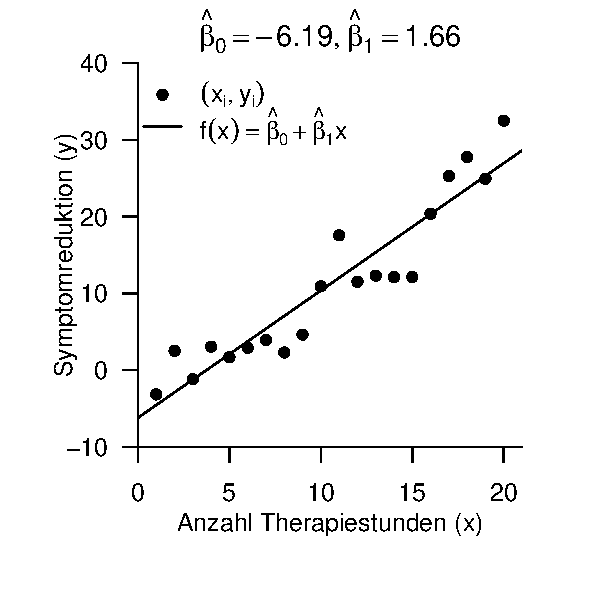
\includegraphics[width=0.55\linewidth]{1_Abbildungen/alm_1_ausgleichsgerade_3} \end{center}
\end{frame}

\begin{frame}{Methode der kleinsten Quadrate}
\protect\hypertarget{methode-der-kleinsten-quadrate-17}{}
\footnotesize
\begin{definition}[Ausgleichspolynom]
\justifying
Für $\beta := (\beta_0,...,\beta_k)^T \in \mathbb{R}^{k+1}$ heißt die Polynomfunktion $k$ten Grades
\begin{equation}
f_\beta : \mathbb{R} \to \mathbb{R}, x \mapsto f_\beta(x) := \sum_{i=0}^k \beta_i x^i,
\end{equation}
für die für eine Wertemenge  $\{(x_1,y_1),...,(x_n,y_n)\} \subset \mathbb{R}^2$ die Funktion
\begin{equation}
q : \mathbb{R}^2 \to \mathbb{R}_{\ge 0}, \beta \mapsto q(\beta)
:= \sum_{i=1}^n \left(y_i-f_\beta(x_i)\right)^2
 = \sum_{i=1}^n \left(y_i- \sum_{i=0}^k \beta_i x^i\right)^2
\end{equation}
der quadrierten vertikalen Abweichungen der $y_i$ von den Funktionswerten
$f_{\beta}(x_i)$ ihr Minimum annimt, das \textit{Ausgleichspolynom $k$ten Grades}
für die Wertemenge $\{(x_1,y_1),...,(x_n,y_n)\}$.
\end{definition}

\footnotesize

Bemerkungen

\begin{itemize}
\tightlist
\item
  Wir nehmen hier ohne Beweis an, dass das Minimum von \(q\) eindeutig
  ist.
\item
  Die Ausgleichsgerade ist das Ausgleichspolynom ersten Grades.
\item
  Die Paramterwerte \(\hat{\beta}_0,...,\hat{\beta}_k\) für die \(q\)
  bei gegebener Wertemenge ihr Minimum annehmen werden an späterer
  Stelle im Rahmen der Theorie des Allgemeinen Linearen Modells ALMs
  bestimmt werden.
\end{itemize}
\end{frame}

\begin{frame}{Methode der kleinsten Quadrate}
\protect\hypertarget{methode-der-kleinsten-quadrate-18}{}
\small

Beispieldatensatz Ausgleichspolynome 1ten bis 4ten Grades

\footnotesize

\begin{center}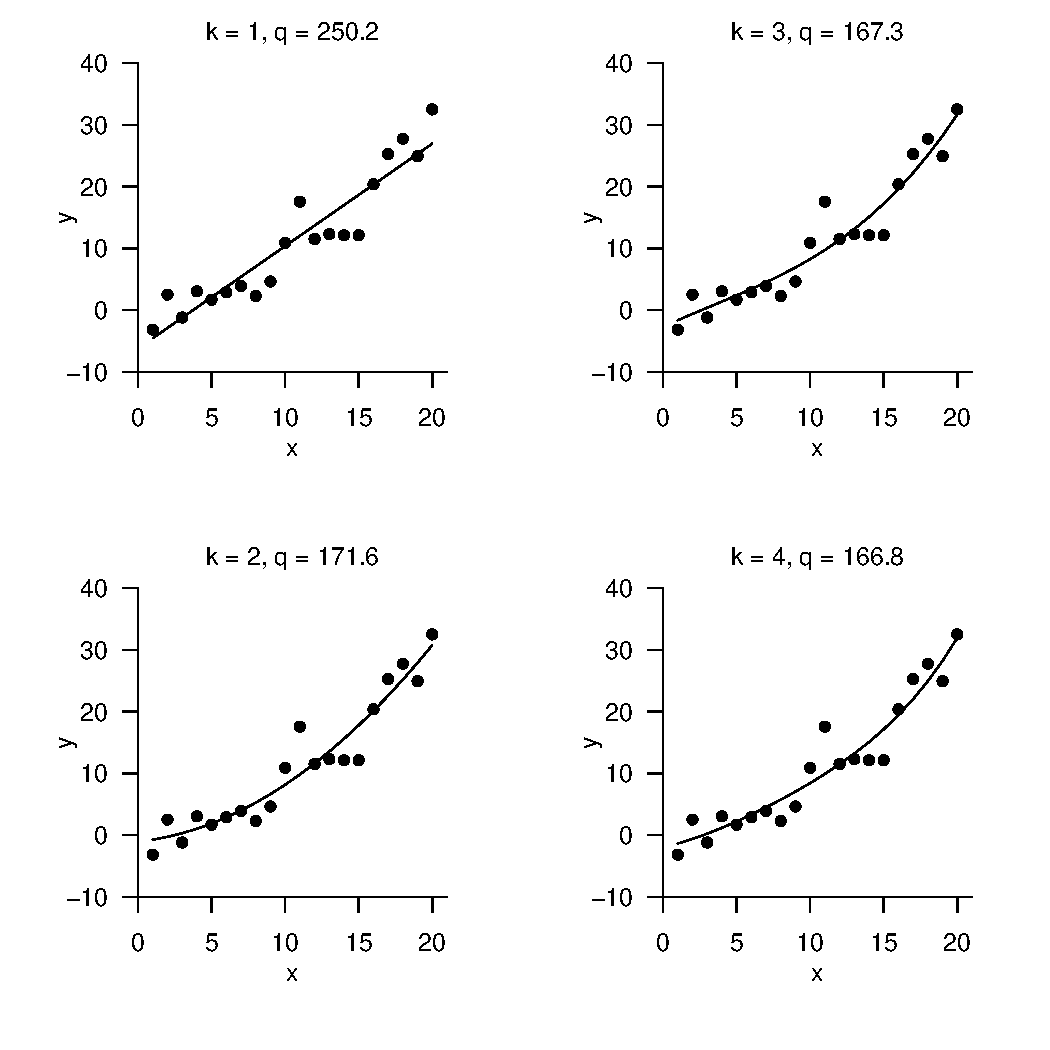
\includegraphics[width=0.6\linewidth]{1_Abbildungen/alm_1_ausgleichspolynom} \end{center}
\vspace{-4mm}
\footnotesize
\center

\(\bullet (x_i, y_i)\) \hspace{2mm} \textbf{---}
\(f_{\hat{\beta}}(x) = \sum_{i=0}^k \hat{\beta}_i x^{i}\)
\end{frame}

\begin{frame}{}
\protect\hypertarget{section-4}{}
\setstretch{3}
\vfill
\large

Methode der kleinsten Quadrate

\textbf{Einfache lineare Regression}

Selbstkontrollfragen

\vfill
\end{frame}

\begin{frame}{Einfache lineare Regression}
\protect\hypertarget{einfache-lineare-regression}{}
Motivation

\justifying
\small

Eine Ausgleichsgerade erlaubt Aussagen über unbeobachtete \(y\) Werte
für \(x\) Werte. Der Wert von \(q(\hat{\beta})\) quantifiziert die Güte
der Ausgleichsgeradenpassung. Eine Ausgleichsgerade erlaubt allerdings
nur implizite Aussagen über die mit der Anpassung verbundene
Unsicherheit.

In der einfachen linearen Regression wird die Idee einer
Ausgleichsgerade um eine probabilistische Komponente (normalverteilte
Fehlervariable) erweitert, um quantitative Aussagen über die mit einer
Ausgleichsgeradenanpassung verbundene Unsicherheit machen zu können.
Weiterhin erlaubt die einfache lineare Regression, einen Hypothesentest-
basierten Zugang zur Einschätzung der angepassten Parameterwerte
\(\hat{\beta}_0\) und \(\hat{\beta}_1\).

Wir betrachten hier zunächst nur das probabilistische Modell der
einfachen linearen Regression sowie die auf ihm basierende Maximum
Likelihood Schätzung der Parameter \(\beta_0\) und \(\beta_1\). Die
Bewertung von Parameterschätzerunsicherheit sowie parameterzentrierte
Hypothesentests behandeln wir an späterer Stelle zunächst im
Allgemeinen.
\end{frame}

\begin{frame}{Einfache lineare Regression}
\protect\hypertarget{einfache-lineare-regression-1}{}
\small
\begin{definition}[Generatives Modell der einfachen linearen Regression]
Für $i = 1,...,n$ sei
\begin{equation}\label{eq:modell_generativ}
Y_i = \beta_0 + \beta_1x_i + \varepsilon_{i}
\end{equation}
wobei
\begin{itemize}
\item $x_i \in \mathbb{R}$ fest vorgegebene sogenannte \textit{Prädiktorwerte} oder \textit{Regressorwerte} sind,
\item $\beta_0,\beta_1 \in \mathbb{R}$ wahre, aber unbekannte, Parameterwerte sind und
\item $\varepsilon_{i} \sim N(0,\sigma^2)$ unabhängige und identisch normalverteilte nicht-beobachtbare Zufallsvariablen mit wahrem, aber unbekanntem, Parameter $\sigma^2 > 0$ sind.
\end{itemize}
Dann heißt \eqref{eq:modell_generativ} \textit{Generatives Modell der einfachen linearen Regression}.
\end{definition}

\footnotesize

Bemerkungen

\begin{itemize}
\tightlist
\item
  Das Modell der einfachen linearen Regression hat drei Parameter,
  \(\beta_0,\beta_1 \in \mathbb{R}\) und \(\sigma^2>0\).
\end{itemize}
\end{frame}

\begin{frame}{Einfache lineare Regression}
\protect\hypertarget{einfache-lineare-regression-2}{}
\small
\begin{theorem}[Normalverteilungsmodell der einfachen linearen Regression]
\normalfont
\justifying
Das generative Modell der einfachen linearen Regression
\begin{equation}\label{eq:modell}
Y_i = \beta_0 + \beta_1x_i + \varepsilon_{i} \mbox{ mit } \varepsilon_i \sim N(0,\sigma^2) \mbox{ u.i.v. für } i = 1,...,n
\end{equation}
lässt sich äquivalent in der Form
\begin{equation}\label{eq:modell_normal}
Y_i \sim N\left(\beta_0 + \beta_1x_i, \sigma^2\right) \mbox{ u.i.v. für } i = 1,...,n
\end{equation}
schreiben.
\end{theorem}

\footnotesize

Bemerkungen

\begin{itemize}
\tightlist
\item
  Wir bezeichnen \begin{equation}
  Y_i \sim N\left(\beta_0 + \beta_1x_i, \sigma^2\right) \mbox{ u.i.v. für } i = 1,...,n
  \end{equation} als
  \textit{Normalverteilungsmodell der einfachen linearen Regression}.
\end{itemize}
\end{frame}

\begin{frame}{Einfache lineare Regression}
\protect\hypertarget{einfache-lineare-regression-3}{}
\tiny
\setlength{\abovedisplayskip}{3pt}
\setlength{\belowdisplayskip}{3pt}
\setstretch{1.2}

\underline{Beweis}

Wir zeigen die Äquivalenz für ein \(i\), die Unabhängigkeit der \(Y_i\)
zeigen wir an späterer Stelle im Rahmen des Allgemeinen Linearen
Modells. Die Äquivalenz beider Modellformen für ein \(i\) folgt direkt
aus der Transformation normalverteilter Zufallsvariablen durch
linear-affine Funktionen (cf.~(8) Transformationen der
Normalverteilung). Speziell gilt im vorliegenden Fall für
\(\varepsilon_i \sim N(0,\sigma^2)\), dass \begin{equation}
Y_i = f(\varepsilon_i)
\mbox{ mit }
f : \mathbb{R} \to \mathbb{R}, \varepsilon_i \mapsto f(\varepsilon_i) := \varepsilon_i + (\beta_0 + \beta_1x_i)
\end{equation} Mit dem WDF Transformationstheorem bei linear-affinen
Abbildungen folgt dann \begin{align}
\begin{split}
p_{Y_i}(y_i)
& = \frac{1}{|1|} p_{\varepsilon_i}\left(\frac{y_i - \beta_0 - \beta_1x_i}{1} \right)       \\
& = N\left(x_i - \beta_0 - \beta_1x_i; 0, \sigma^2\right)                                   \\
& = \frac{1}{\sqrt{2\pi\sigma^2}}\exp\left(-\frac{1}{2\sigma^2}(x_i - \beta_0 - \beta_1x_i - 0)^2 \right)    \\
& = \frac{1}{\sqrt{2\pi\sigma^2}}\exp\left(-\frac{1}{2\sigma^2}(x_i - (\beta_0 + \beta_1x_i)^2 \right)        \\
& = N\left(x_i; \beta_0 + \beta_1x_i,\sigma^2\right),
\end{split}
\end{align} also \begin{equation}
Y_i \sim N\left(\beta_0 + \beta_1x_i,\sigma^2\right).
\end{equation}
\end{frame}

\begin{frame}{Einfache lineare Regression}
\protect\hypertarget{einfache-lineare-regression-4}{}
Modell der einfachen linearen Regression \vspace{1mm} \setstretch{1.2}

\begin{center}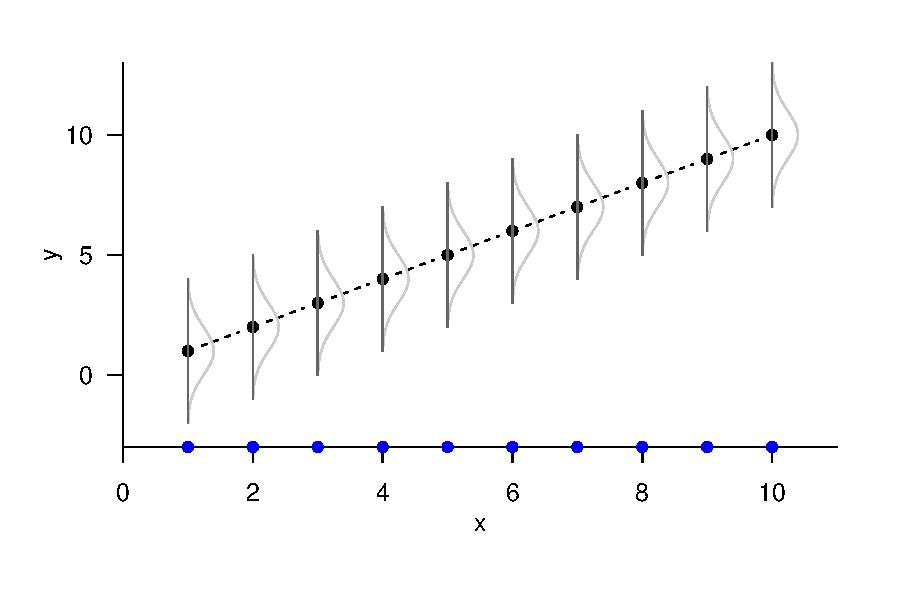
\includegraphics[width=0.85\linewidth]{1_Abbildungen/alm_1_elr_1} \end{center}
\vspace{-4mm}
\footnotesize
\center

\textcolor{blue}{$\bullet$} \(x_i\) \hspace{2mm} \(\bullet\)
\(\beta_0 + \beta_1x_i\) \mbox{ für } \(\beta_0 := 0\), \(\beta_1 := 1\)
\hspace{2mm} \textcolor{gray}{\textbf{---}}
\(N(y_i; \beta_0 + \beta_1x_i, \sigma^2)\) \mbox{ für }
\(\sigma^2 := 1\).
\end{frame}

\begin{frame}{Einfache lineare Regression}
\protect\hypertarget{einfache-lineare-regression-5}{}
Realisierung des Modells der einfachen linearen Regression \vspace{1mm}
\setstretch{1.2}

\begin{center}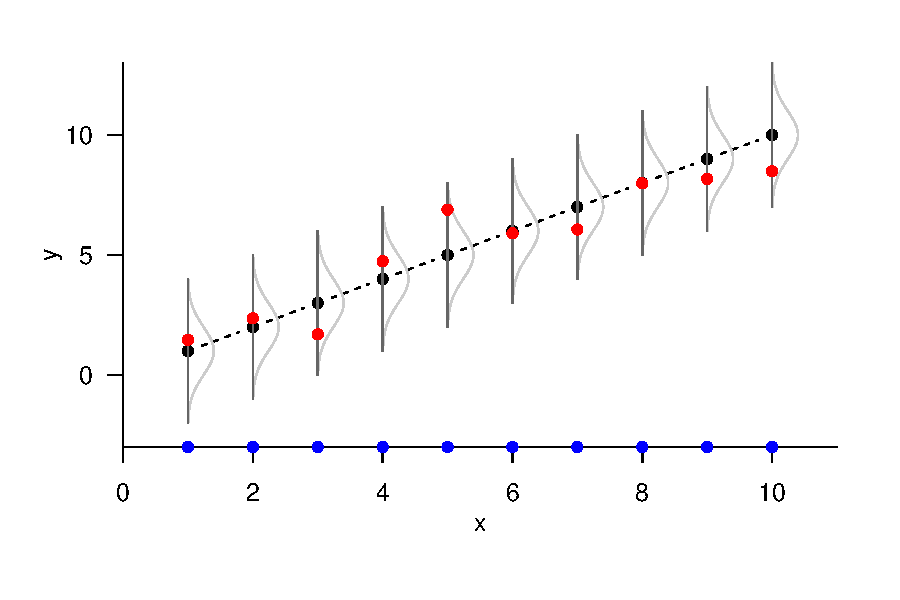
\includegraphics[width=0.85\linewidth]{1_Abbildungen/alm_1_elr_2} \end{center}
\vspace{-4mm}
\footnotesize
\center

\textcolor{blue}{$\bullet$} \(x_i\) \hspace{2mm} \(\bullet\)
\(\beta_0 + \beta_1x_i\) \mbox{ für } \(\beta_0 := 0\), \(\beta_1 := 1\)
\hspace{2mm} \textcolor{gray}{\textbf{---}}
\(N(y_i; \beta_0 + \beta_1x_i, \sigma^2)\) \mbox{ für }
\(\sigma^2 := 1\) \hspace{2mm} \textcolor{red}{$\bullet$} \((x_i,y_i)\)
\end{frame}

\begin{frame}{Einfache lineare Regression}
\protect\hypertarget{einfache-lineare-regression-6}{}
\small
\begin{theorem}[Maximum Likelihood Schätzung]
\justifying
\normalfont
Es sei
\begin{equation}\label{eq:modell}
Y_i = \beta_0 + \beta_1x_i + \varepsilon_{i} \mbox{ mit } \varepsilon_i \sim N(0,\sigma^2) \mbox{ u.i.v. für } i = 1,...,n
\end{equation}
das Modell der einfachen linearen Regression. Dann sind Maximum Likelihood
Schätzer der Modellparameter $\beta_0,\beta_1$ und $\sigma^2$ gegeben durch
\begin{equation}
\hat{\beta}_1  := \frac{c_{xy}}{s_x^2}, \,\,\,
\hat{\beta}_0  := \bar{y} - \hat{\beta}_1\bar{x} \,\,\,
\mbox{ und }
\hat{\sigma}^2 := \frac{1}{n}\sum_{i=1}^n \left(y_i - \left(\hat{\beta}_0 + \hat{\beta}_1 x_i\right)\right)^2.
\end{equation}
\end{theorem}

\footnotesize

Bemerkungen

\begin{itemize}
\tightlist
\item
  Wir verzichten hier aus Gründen der Übersichtlichkeit auf die
  \(^{\tiny \mbox{ML}}\) Superskripte.
\item
  Die ML Schätzer für \(\beta_0\) und \(\beta_1\) sind offenbar mit den
  Ausgleichsgeradenparametern identisch.
\end{itemize}
\end{frame}

\begin{frame}{Einfache lineare Regression}
\protect\hypertarget{einfache-lineare-regression-7}{}
\tiny
\setlength{\abovedisplayskip}{1pt}
\setlength{\belowdisplayskip}{1pt}

\underline{Beweis}

Wir zeigen zunächst, dass die Ausgleichsgerardenparameter
\(\hat{\beta}_0\) und \(\hat{\beta}_1\) den entsprechenden ML Schätzern
gleichen. Dazu halten wir zunächst fest, dass aufgrund der
Unabhängigkeit der \(Y_1, ...,Y_n\) die Likelihood-Funktion des Modells
der einfachen linearen Regression bezüglich \(\beta_0\) und \(\beta_1\)
die Form \begin{align}
\begin{split}
L : \mathbb{R}^2 \to \mathbb{R}_{>0}, (\beta_0,\beta_1) \mapsto L(\beta_0,\beta_1)
& := \prod_{i=1}^n \frac{1}{\sqrt{2\pi\sigma^2}}\exp\left(-\frac{1}{2\sigma^2}(y_i - (\beta_0 + \beta_1x_i))^2\right) \\
&  = \left(2\pi\sigma^2\right)^{-\frac{n}{2}}\exp\left(-\frac{1}{2\sigma^2}\sum_{i=1}^n(y_i - (\beta_0 + \beta_1x_i))^2\right)
\end{split}
\end{align} Weil für die Exponentialfunktion gilt, dass für
\(a < b \le 0\) gilt, dass \(\exp(a)<\exp(b)\) wird der Exponentialterm
dieser Likelihood-Funktion maximal, wenn der Term
\begin{equation}\label{eq:q}
q := \sum_{i=1}^n(y_i - (\beta_0 + \beta_1x_i))^2 \ge 0
\end{equation} minimal und damit \(-q\) maximal wird. Im Rahmen des
Beweises der Ausgleichsgeradenform haben wir aber schon gezeigt, dass
der Term \eqref{eq:q} für \begin{equation}
\hat{\beta}_1   := \frac{c_{xy}}{s_x^2} \mbox{ und } \hat{\beta}_0   := \bar{y} - \hat{\beta}_1\bar{x}
\end{equation} minimal wird, und damit \(\hat{\beta}_1\) und
\(\hat{\beta}_0\) die Likelihood-Funktion maximieren.
\end{frame}

\begin{frame}{Einfache lineare Regression}
\protect\hypertarget{einfache-lineare-regression-8}{}
\tiny
\setlength{\abovedisplayskip}{1pt}
\setlength{\belowdisplayskip}{1pt}

\underline{Beweis (fortgeführt)}

In einem zweiten Schritt betrachten wir nun die Likelihood-Funktion des
Modells der einfachen linearen Regression bezüglich \(\sigma^2\) an der
Stelle von \(\hat{\beta}_0\) und \(\hat{\beta}_1\). Wir erhalten die
Likelihood-Funktion \begin{equation}
L : \mathbb{R}_{>0} \to \mathbb{R}_{>0}, \sigma^2 \mapsto L(\sigma^2)
 = \left(2\pi\sigma^2\right)^{-\frac{n}{2}}\exp\left(-\frac{1}{2\sigma^2}\sum_{i=1}^n(y_i - (\hat{\beta}_0 + \hat{\beta}_1x_i))^2\right)
\end{equation} und die entsprechende Log-Likelihood-Funktion
\begin{equation}
\ell : \mathbb{R}_{>0} \to \mathbb{R}, \sigma^2 \mapsto \ell(\sigma^2)
 = -\frac{n}{2} \ln 2\pi - \frac{n}{2} \ln \sigma^2 -\frac{1}{2\sigma^2}\sum_{i=1}^n(y_i - (\hat{\beta}_0 + \hat{\beta}_1x_i))^2
\end{equation} In Analogie zu der Herleitung des ML Schätzers für
\(\sigma^2\) im Normalverteilungsmodell (cf.~(10) Parameterschätzung)
ergibt sich unter Beachtung von \begin{equation}
\hat{\mu}^{\mbox{\tiny ML}}_n = \hat{\beta}_0 + \hat{\beta}_1x_i
\end{equation} dann hier \begin{equation}
\hat{\sigma}^2 = \frac{1}{n}\sum_{i=1}^n (y_i - (\hat{\beta}_0 + \hat{\beta}_1x_i))^2.
\end{equation}
\end{frame}

\begin{frame}[fragile]{Einfache lineare Regression}
\protect\hypertarget{einfache-lineare-regression-9}{}
Beispieldatensatz Parameterschätzung \vspace{2mm} \setstretch{1}

\tiny

\begin{Shaded}
\begin{Highlighting}[]
\CommentTok{\# Einlesen des Beispieldatensatzes}
\NormalTok{fname       }\OtherTok{=} \FunctionTok{file.path}\NormalTok{(}\FunctionTok{getwd}\NormalTok{(), }\StringTok{"1\_Daten"}\NormalTok{, }\StringTok{"1\_Regression.csv"}\NormalTok{)}
\NormalTok{D           }\OtherTok{=} \FunctionTok{read.table}\NormalTok{(fname, }\AttributeTok{sep =} \StringTok{","}\NormalTok{, }\AttributeTok{header =} \ConstantTok{TRUE}\NormalTok{)}

\CommentTok{\# Stichprobenstatistiken}
\NormalTok{n           }\OtherTok{=} \FunctionTok{length}\NormalTok{(D}\SpecialCharTok{$}\NormalTok{y\_i)                                      }\CommentTok{\# Anzahl Datenpunkte}
\NormalTok{x\_bar       }\OtherTok{=} \FunctionTok{mean}\NormalTok{(D}\SpecialCharTok{$}\NormalTok{x\_i)                                        }\CommentTok{\# Stichprobenmittel der x\_i{-}Werte}
\NormalTok{y\_bar       }\OtherTok{=} \FunctionTok{mean}\NormalTok{(D}\SpecialCharTok{$}\NormalTok{y\_i)                                        }\CommentTok{\# Stichprobenmittel der y\_i{-}Werte}
\NormalTok{s2x         }\OtherTok{=} \FunctionTok{var}\NormalTok{(D}\SpecialCharTok{$}\NormalTok{x\_i)                                         }\CommentTok{\# Stichprobenvarianz der  x\_i{-}Werte}
\NormalTok{cxy         }\OtherTok{=} \FunctionTok{cov}\NormalTok{(D}\SpecialCharTok{$}\NormalTok{x\_i, D}\SpecialCharTok{$}\NormalTok{y\_i)                                  }\CommentTok{\# Stichprobenkovarianz der (x\_i,y\_i){-}Werte}

\CommentTok{\# Parameteterschätzer}
\NormalTok{beta\_1\_hat  }\OtherTok{=}\NormalTok{ cxy}\SpecialCharTok{/}\NormalTok{s2x                                            }\CommentTok{\# \textbackslash{}hat\{\textbackslash{}beta\}\_1, Steigungsparameter}
\NormalTok{beta\_0\_hat  }\OtherTok{=}\NormalTok{ y\_bar }\SpecialCharTok{{-}}\NormalTok{ beta\_1\_hat}\SpecialCharTok{*}\NormalTok{x\_bar                           }\CommentTok{\# \textbackslash{}hat\{\textbackslash{}beta\}\_0, Offset Parameter}
\NormalTok{sigsqr\_hat  }\OtherTok{=}\NormalTok{ (}\DecValTok{1}\SpecialCharTok{/}\NormalTok{n)}\SpecialCharTok{*}\FunctionTok{sum}\NormalTok{((D}\SpecialCharTok{$}\NormalTok{y\_i}\SpecialCharTok{{-}}\NormalTok{(beta\_0\_hat}\SpecialCharTok{+}\NormalTok{beta\_1\_hat}\SpecialCharTok{*}\NormalTok{D}\SpecialCharTok{$}\NormalTok{x\_i))}\SpecialCharTok{\^{}}\DecValTok{2}\NormalTok{) }\CommentTok{\# Varianzparameter}


\CommentTok{\# Ausgabe}
\FunctionTok{cat}\NormalTok{(}\StringTok{"beta\_0\_hat:"}\NormalTok{  , beta\_0\_hat,}
    \StringTok{"}\SpecialCharTok{\textbackslash{}n}\StringTok{beta\_1\_hat:"}\NormalTok{, beta\_1\_hat,}
    \StringTok{"}\SpecialCharTok{\textbackslash{}n}\StringTok{sigsqr\_hat:"}\NormalTok{, }\FunctionTok{sqrt}\NormalTok{(sigsqr\_hat))}
\end{Highlighting}
\end{Shaded}

\begin{verbatim}
> beta_0_hat: -6.19 
> beta_1_hat: 1.66 
> sigsqr_hat: 3.54
\end{verbatim}
\end{frame}

\begin{frame}[fragile]{Einfache lineare Regression}
\protect\hypertarget{einfache-lineare-regression-10}{}
Beispieldatensatz Analyse mit \texttt{lm()} \vspace{1mm}
\setstretch{1.2}

\tiny

\begin{Shaded}
\begin{Highlighting}[]
\CommentTok{\# Einlesen des Beispieldatensatzes}
\FunctionTok{library}\NormalTok{(car)}
\end{Highlighting}
\end{Shaded}

\begin{verbatim}
> Lade nötiges Paket: carData
\end{verbatim}

\begin{Shaded}
\begin{Highlighting}[]
\NormalTok{fname       }\OtherTok{=} \FunctionTok{file.path}\NormalTok{(}\FunctionTok{getwd}\NormalTok{(), }\StringTok{"1\_Daten"}\NormalTok{, }\StringTok{"1\_Regression.csv"}\NormalTok{)}
\NormalTok{D           }\OtherTok{=} \FunctionTok{read.table}\NormalTok{(fname, }\AttributeTok{sep =} \StringTok{","}\NormalTok{, }\AttributeTok{header =} \ConstantTok{TRUE}\NormalTok{)}

\CommentTok{\# Analyse mit lm()}
\NormalTok{model       }\OtherTok{=} \FunctionTok{lm}\NormalTok{(}\AttributeTok{formula =}\NormalTok{ D}\SpecialCharTok{$}\NormalTok{y\_i }\SpecialCharTok{\textasciitilde{}}\NormalTok{ D}\SpecialCharTok{$}\NormalTok{x\_i, }\AttributeTok{data =}\NormalTok{ D)}
\FunctionTok{print}\NormalTok{(model)}
\end{Highlighting}
\end{Shaded}

\begin{verbatim}
> 
> Call:
> lm(formula = D$y_i ~ D$x_i, data = D)
> 
> Coefficients:
> (Intercept)        D$x_i  
>       -6.19         1.66
\end{verbatim}
\end{frame}

\begin{frame}{}
\protect\hypertarget{section-5}{}
\setstretch{3}
\vfill
\large

Methode der kleinsten Quadrate

Einfache lineare Regression

\textbf{Selbstkontrollfragen}

\vfill
\end{frame}

\begin{frame}{References}
\protect\hypertarget{references}{}
\footnotesize
\end{frame}

\end{document}
